\subsubsection{Yorkshire Brawl}

\paragraph{Outline}

Yorkshire Brawl is a more chaotic version of French Brawl. FB is restricted, smaller map, less bonuses, YB has the same settings with a fully open map so important territories that control regions + safe FTBs + expansion is the way.
\\
\\
The borders aren't that well balanced. Harrogate (Orange +2 center) influences within 1 turn a dozen different bonuses with decent borders on top. The west is harder to defend due to that, once your opponent gets in Harrogate, it's gg. The east is more spread out with linear bonuses that you can never get recaptured at. South is usually ignored as the the +4 requires a triple pick, and North Lincolnshire/Doncaster are one-dimensional.

\paragraph{Gameplay}

Really, YB in picks is a lot about prioritizing safe FTBs/combos and covering not-so-safe FTBs/combos while trying to have as high as possible good territories. On the latter, \href{https://www.warzone.com/MultiPlayer?GameID=40069574}{Octane's FP} in this game is an all-around pick in that it can be used as a combo for 5 different bonuses and defensively shields potentially his own bonuses. As seen on T1, Octane has a dynamic of 2vs4 picks on the north that threaten everything Jake can complete.
\\
\\
By saying prioritize FTBs, for example \href{https://www.warzone.com/MultiPlayer?GameID=38982476}{here} me and Octane mirror 1/2 and 3/4 due to how we want maximum presence in the areas. \href{https://www.warzone.com/MultiPlayer?GameID=40721173}{Here} both Octane and Xeno mirror the +1 FTB west into investing towards the +2 FTBs in the center in a different order. Order of picks + gameplay define the template, nothing is standard.
\\
\\
On picks and gameplay in unclear setups, \href{https://www.warzone.com/MultiPlayer?GameID=35335475}{in this distribution}:
\begin{enumerate}
    \item Try to simplify the position and eliminate some picks from eligibility. There's $\sim$ 8 territories I evaluate as ones you can't skip/have to play around, and another 10 more that fill in depending on order of picks and strategy. But at the end, you need a set of 12 picks, see Figure \ref{yb_board}.
\begin{figure}[H]
  \centering
  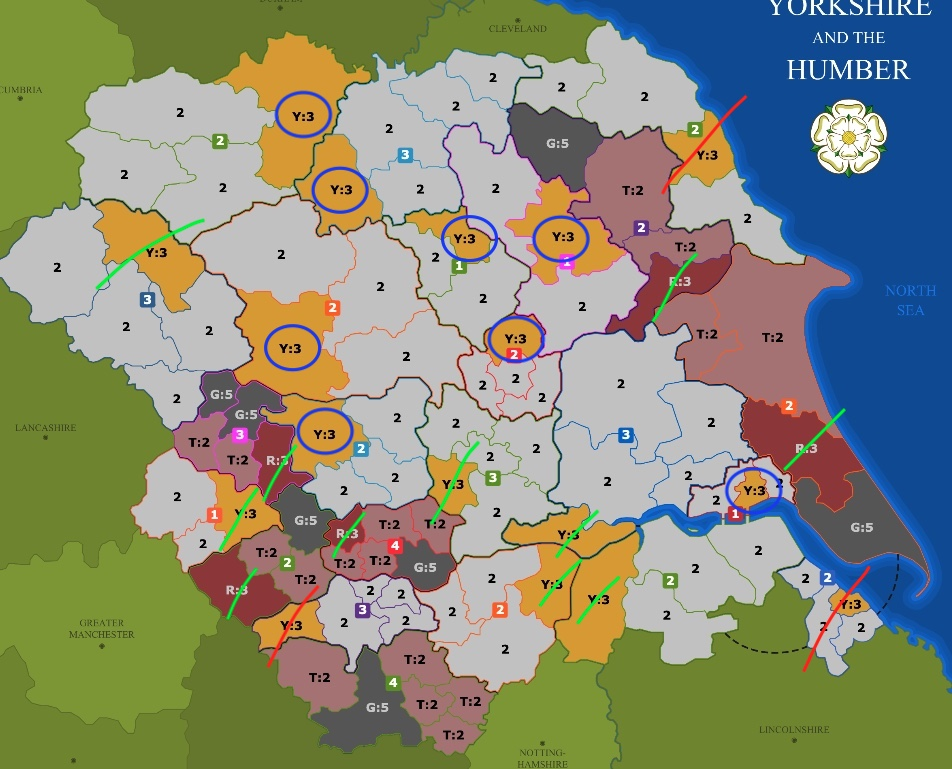
\includegraphics[width=0.8\textwidth]{Images/yb_board.jpg}
  \caption{Distribution. Y3:Neutrals in Distribution. R3: Neutrals in Distribution in Wastelanded bonuses, G5/T2:Wastelanded territories/Bonuses. Blue circles: Higher priority territories. Light Green line: Situational. Red Line: Discard.}
  \label{yb_board}
\end{figure}
    \item The North comes with 3 +2 FTBs and 2 +1 FTBs. Besides that there's an FTB +1 in the West and slow income South. The principled way to approach such a position includes either committing fully to the brawl North or just covering the brawl north with positional picks and prioritizing safer income.
    \item First thing to identify from mod's picks is that he recognizes how the edges are less useful than his 1-4 picks, and secondly losing 3/4/5 guarantees 6 as a counter with first order T1. Losing 3/4 and getting 1/2/5 allows him to get double border vs FTB with extra armies. Given you can connect the armies at the +1s to control the +2 FTB as well as just get the +1 FTBs in the first place, that region is better. The players deviate after prioritizing the North cluster to different ideas, Crazy embracing the brawl, mod going for safe income.
    \item Pause end of Turn 2. 7vs7, 13vs10 territories. I think Crazy's win condition is out-delaying mod and forcing eliminations North the moment mod tries to expand because Crazy's income comes from his territories and he is at 2vs3 usable armies North at the moment. In his shoes T3 with first order, imo you should +1 somewhere in the pink +1 and tap mod's territory to get a favorable 1:1 trade and grab one of mod's delays). From mod's pov, the game end of t2 and till however long it takes, is about stabilizing in the north, getting good kill-rates, and punishing mistakes. Going through the moves you can see exactly that with Crazy wasting 1 army in a 1:0 tap on T3 and 2 more armies on 1:0 taps on T4 that result by the end of T4 in a 7vs7 Income and 13vs11 territories position with mod having 2 armies advantage.
    \begin{itemize}
        \item end of T2 7vs7, 13vs10 terr, 2vs3 movable armies 
        \item end of T4 7vs7, 13vs11 terr, 0vs3 movable armies
    \end{itemize}
    \item This is the main take away for the messy distributions, the question of how to play your position which is exclusively kill-rates, playing with the move-order, meaningful taps and forcing your opponent to waste armies. Those two turns gave enough edge to mod to pivot south for more income, temporarily sacrificing his position north, while Crazy now has to gamble on T5 2-army attacks everywhere due to the threat of expansion south
\end{enumerate}

On specific games, from my experience YB is more random than FB both in picks and gameplay, sometimes requiring very bold moves that can be coin-flippy. The way I approach it:
\begin{enumerate}
    \item \href{https://www.warzone.com/MultiPlayer?GameID=41377144}{7ate9 vs Stales78}, I pick for coverage, no specific idea for T1 in mind. 1/3 to cover 3 FTBs east and bait more opponents by the opponent, 2/4 center presence on +2 FTBs/combos, 5/6 versatily combo +2/+1 and cover of the +3 above it, 7 to pair with 1/3, 8-11 fill with adjacent (11 to pair with 2/3) and 12 troll. I get a winning position T2 (should've went for 14 terr, split attack 3/3 west to capture back and border the +3), fumble it T3 in a way unimaginably to the human mind, somehow make a comeback T4 and then forget to reorder my moves T5 into a tilt surrender. I think my picks approach up to 7th is better but I got outplayed. But seeing this in retrospect, even a 7th pick there is a misplay given with my set I can lose 1/5/6/8 as SP.
    \item \href{https://www.warzone.com/MultiPlayer?GameID=41343286}{7ate9 vs Mr.Carpenter}, I missed the idea that I can get the +1 west with 0 deploys and 2 taps. Misplayed t1, misplayed t3, pointless to attack, lost a territory and fell to 11 territories, and from there it's an uphill battle. 
    \item \href{https://www.warzone.com/MultiPlayer?GameID=41343983}{7ate9 vs Rufus}, it's a board with a trillion +2 FTBs and impossible to cover everything. North East +2 FTB is the safest but 0 expansion and 3pick committment in a rich board -> Ignore. South +2 FTB is great safe with expansion, but I don't like the isolated picks. West Green +2 FTB comes with Calderdale +1 FTB and all sorts of counters. Rich in income area, even my 11th counters everything, and the +4. Got a lucky outcome in picks as Rufus had the idea of 9-11 cover south, and he never reached his 9th into into a prediction due to the threat of the +4.
    \item \href{https://www.warzone.com/MultiPlayer?GameID=39713419}{vs Guest} the game end of T1 is about finding a way to get Guest <10 territories. That's my win condition, as I'm completing the +2 Bonus and can convert a 7vs6 or 6vs5 income game. \href{https://www.warzone.com/MultiPlayer?GameID=39755538}{vs Forsaken} the game is won on picks. I did get his first pick but even if we reverse mo, I get 2 picks west. \href{https://www.warzone.com/MultiPlayer?GameID=38007899}{vs Poldi} playing from behind and expanding to match the opponent's income.
\end{enumerate}


%wastelanded bonuses are generally stronger due to the map being more balaced. (stronger than fb).

%\href{https://www.warzone.com/MultiPlayer?GameID=35276995}{train} on how to pick in yorkshire brawl + chat

%\href{https://www.warzone.com/MultiPlayer?GameID=35277140}{train2} the less picks contesting a bonus the better it is. + advice in chat

%If you can only find 10 or 11 picks, make your last picks ones that can immediately transfer to another so they can be useful.

